\section{Materiales y métodos}

En este apartado se explicará los diferentes métodos que se han seguido a lo largo de un proceso para la reutilización de fármacos.

El inicio de nuestra investigación se ha basado leyendo un número de artículos para ponernos en situación del virus SARS-CoV-2. Encontramos en unos de los paper \cite{Gordon2020}, que el virus forma 29 proteínas, pero que tan solo han sido clonadas y expresadas 26 proteínas de las 29.  Estas 26, las señaladas en la tabla 1, son las usada en la investigación y con las que será generado el interactoma proteínas humanas-SARS-Cov-2. 


\subsection{STRING, Protein-Protein Interaction Networks}

Visto anteriormente, la principal idea es obtener que relaciones tienen las proteínas del virus con nuestro cuerpo. De esta manera, sabremos con que proteínas humanas interactúan y así encontrar fármacos que afecten directamente a ellas. El pensamiento es que estos fármacos eviten en cierta medida, la clonación y la infección del virus de manera indirecta. 

Para encontrar las proteínas secundarias, llamadas de esta forma en los artículos leídos, se hará uso de la base de datos STRING. 
STRING se usa para obtener las relaciones de las proteínas del SARS-Cov-2, con todas las humanas. Las proteínas humanas mostradas en STRING son 332 que serán clave en la investigación de los fármacos. 

\subsection{redSring.R}

Una vez hecho la búsqueda de las 332 proteínas humanas, las guardamos en un fichero de entrada. Posteriormente este archivo, creará un mapeo de estas mismas proteínas, pero queriendo reducir el número de ellas. 

El archivo ejecutará un mapeo sobre las 332 proteínas humanas encontradas en STRING. Utilizará el fichero donde vienen las proteínas y creará un dataframe donde vendrán el nombre de las proteínas y además se añadirá una columna con STRINGID de cada una de ellas. Después, la intención es obtener una subred de las interacciones entre esas 332, para generar una red secundaria de las interacciones más fuertes. Para ello hemos utilizado un combined score mayor a 900. 

Este proceso se utiliza, porque nos ayudará a tener unos resultados más fiables a la hora de encontrar fármacos. Debido a que encontraremos fármacos que afecten a relaciones muy estrechas. 

\subsection{convertirUniprot.R}

Este fichero es auxiliar. Nos va a ayudar a convertir los Gene Name de las proteinas obtenidas en el archivo redString.R, en su nombre de UniProt. Por lo que, devolverá un fichero .txt con los respectivos nombres. 

Se realiza esta conversión, para tener los datos preparados en la búsqueda de fármacos en CHEMBL. 

\subsection{Bases de datos CHEMBL y fichero consultarChembl.py}

    \subsubsection{Bases de datos CHEMBL y consultas en Myqsl}
    En el informe de la explicación de la práctica, nos dice que: Las proteínas humanas con las que interaccionan las proteínas virales de SARSCoV2 pueden ser targets farmacológicos de interés, por lo que en este proyecto se pretende encontrar fármacos de la base de datos ChEMBL que tengan como diana las proteínas o módulos del interactoma funcional SARS-humano. Por lo tanto, todo lo que se ha hecho hasta ahora es facilitar el trabajo para que una vez hayamos obtenidos esos denominados targets, se busquen en esta bases de datos. 
    
    ChEMBL tiene la posibilidad de ser descargada en diferentes formatos para ser trabajada desde Oracle, MySQL, XML, etc. La base de datos ChEMBL ha sido descargada en formato MySQL para realización del informe. Mediante un esquema de las tablas proporcionadas y una guía donde explica cada tabla y cada elemento, hemos podido hacer la consulta sobre los fármacos que queremos. Hemos realizado una ruta entre las tablas que necesitamos acordes con los datos preparados. 
    
    La consulta en cuestión es: 
    
		\begin{figure}[h!]
			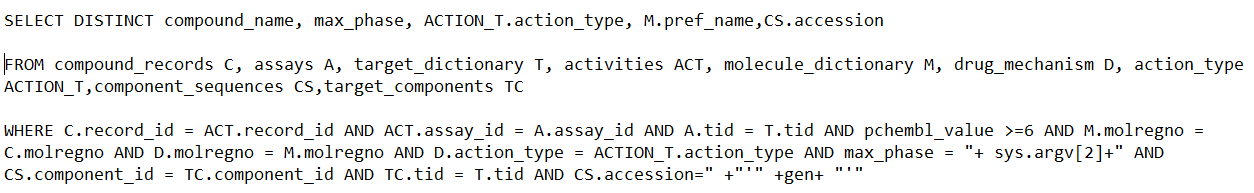
\includegraphics[width=0.9\textwidth]{figures/Captura.PNG}
			\caption{Consulta MySQL}
			\label{fig:cost_megabase}
		\end{figure}
	\newpage
		
	Tal y como podemos ver en esta consulta, accedemos a varias tablas de la base de datos. Para explicar esto mejor, vamos a mostrar el esquema de la base de datos de Chembl, pero únicamente las tablas que hemos utilizado:
    
    \begin{figure}[h!]
			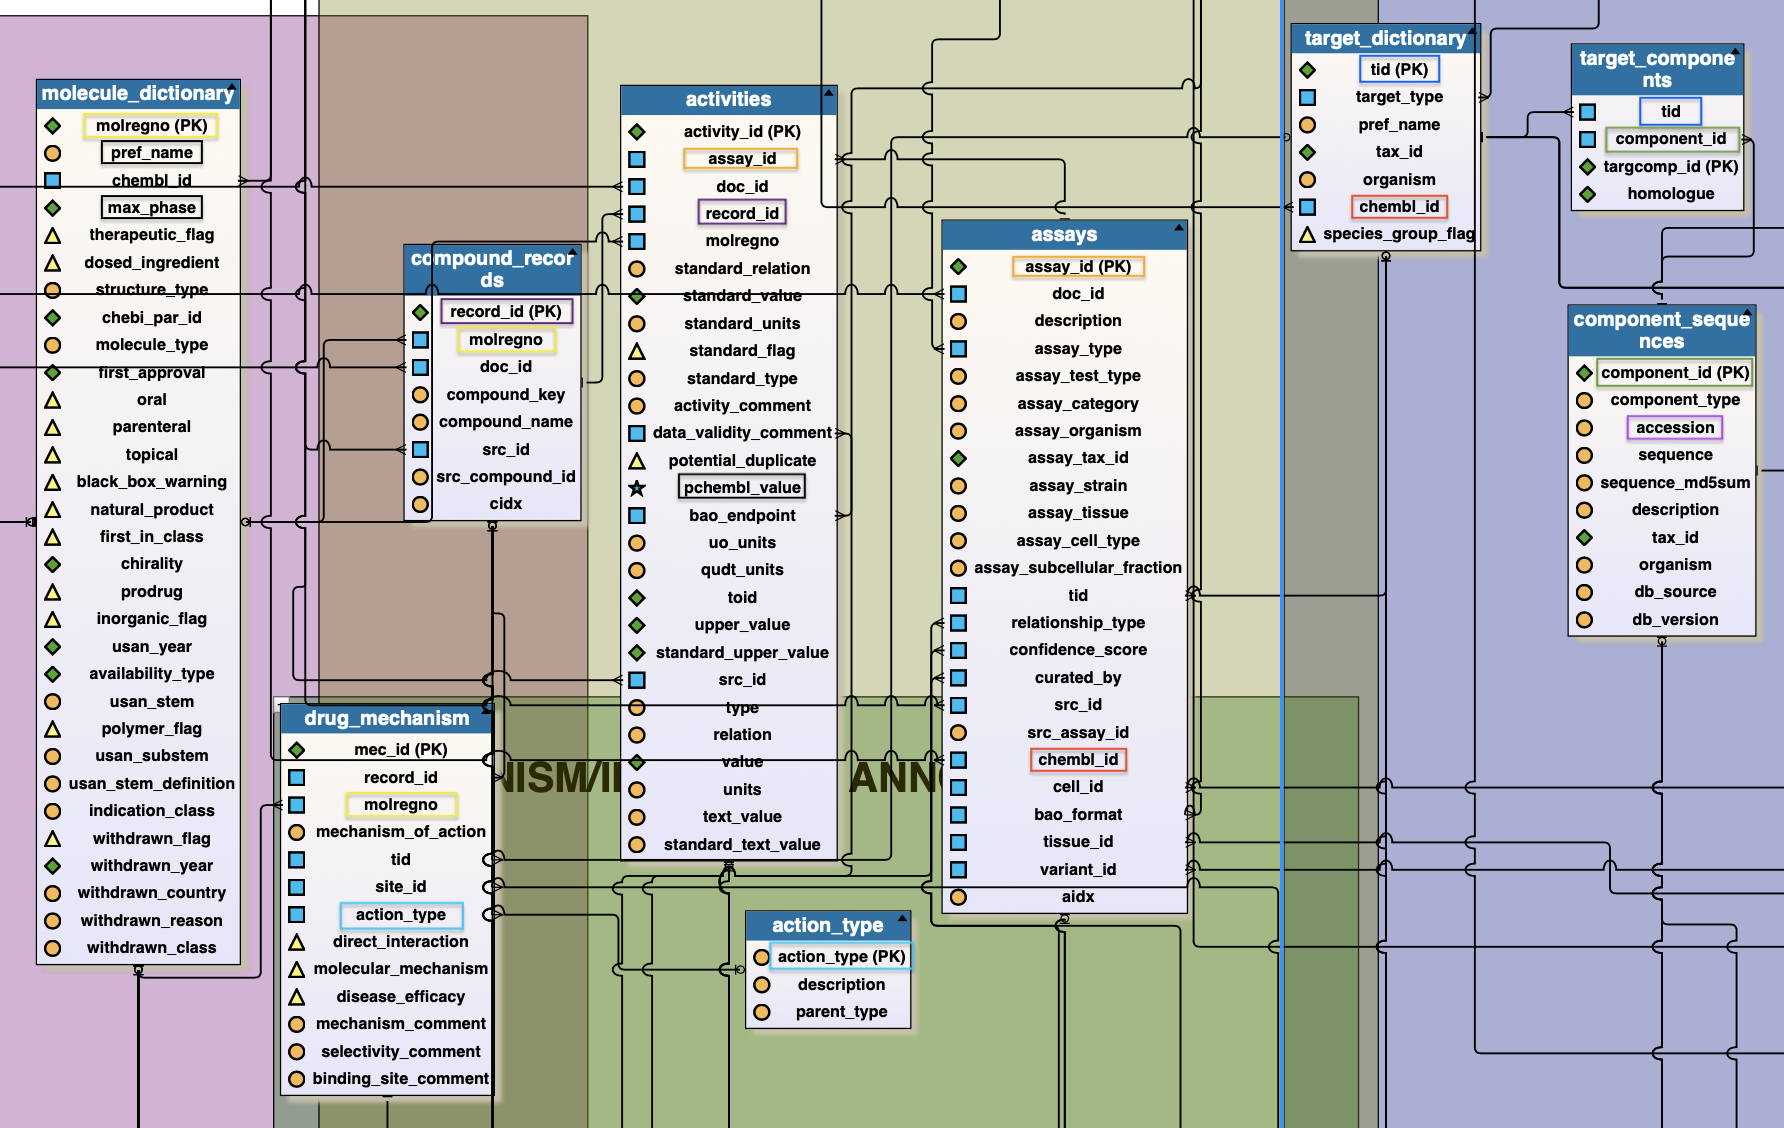
\includegraphics[width=0.9\textwidth]{figures/esquema.png}
			\caption{Esquema Chembl DB}
			\label{fig:cost_megabase}
		\end{figure}
	
    Accedemos a este esquema por el atributo \textbf{accession} de la tabla \textbf{component sequences}, en las que introducimos el UniprotID de las 178 proteínas humanas que hemos extraído anteriormente.  
    
    Desde ahí, recorremos un camino, marcado en la figura con recuadros en los atributos de cada tabla, en el que pasamos por la tabla \textbf{target components} a través del component id de la proteínas, cogemos el tid y llegamos a la tabla \textbf{target dictionary}, de donde sacaremos el Chembl ID de la proteína para llegar a la tabla \textbf{assays}.  
    
    Con el assay id accedemos a la tabla \textbf{activities}, que además de formar parte de la ruta desde la proteína hasta sus fármacos asociados, contiene el valor de P Chembl, que vamos a utilizar para filtrar los fármacos: con un P Chembl value mayor a 6 nos aseguramos que los compuestos estén estrechamente relacionados con las proteínas. En esta misma tabla, nos encontramos el record id, que nos servirá para enlazar con la tabla \textbf{compound records}, nuestro objetivo. 
    
    Una vez llegados aquí, ya tenemos la lista de fármacos asociados, pero hemos indagado más, recurriendo a las tablas \textbf{molecule dictionary}, \textbf{drug mechanism} y \textbf{action type} para incluir en nuestra consulta, además, el tipo de acción que ejerce el fármaco, la fase de ensayo en la que se encuentra (que hemos dividido en fármacos experimentañes, fase 3, y fármacos aprobados, fase 4) y el nombre común que tienen los compuestos, ya que el científico resultaba muy poco evidente.
    
    
    \subsubsection{Código en python. consultarChembl.py}
    Debido al gran número de proteínas obtenidas, sería muy costoso y lento ir buscando en la consulta de MySQL una a una. Por lo que, se ha creado un programa Python, que lee el fichero donde se encuentran las 178 proteínas con sus respectivos nombres y UniProt ID.
    
    El programa se conecta a las bases de datos descargada en el ordenador y procede a hacer un bucle leyendo cada línea del fichero. De esta manera, va leyendo cada UniProt ID y la va introduciendo en la consulta para ir obteniendo nuestro resultado final que sería los fármacos que estábamos buscando al inicio de la investigación. 
    
    Se ha decidido que los fármacos buscados sean del tipo 3 y 4. Donde el tipo 3 son fármacos experimentales y de tipo 4 fármacos aprobados. Esta decisión es debida a que así tendremos una certeza adecuada de funcionalidad del fármaco hallado. 

    
    
\subsection{analisisResultados.R}
La ejecución de este fichero sirve para obtener graficas sobre los fármacos encontrados y poder evaluar los resultados obtenidos. 
El arvicho que recoge el fichero es el obtenido en el programa de Python. 

\subsection{launch.sh}
Es un flujo del trabajo completo, el fichero que hay que ejecutar para que se lleve a cabo todo el proceso. Es el fichero principal, un flujo bash

